\documentclass[border=10pt]{standalone}
% Shared style for the EMONI diagrams. Build: tectonic <file>.tex, then pdftocairo -svg.
\usepackage{fontspec}
\setmainfont{FiraSans}[Extension=.otf,UprightFont=*-Regular,BoldFont=*-SemiBold,ItalicFont=*-Italic,BoldItalicFont=*-SemiBoldItalic]
\setmonofont{FiraMono}[Extension=.otf,UprightFont=*-Regular,BoldFont=*-Medium,Scale=0.9]
\usepackage{tikz}
\usetikzlibrary{arrows.meta,positioning,shapes.geometric,shapes.misc,calc,fit,backgrounds}
\definecolor{eg}{HTML}{11903B}   % EMONI green
\definecolor{egl}{HTML}{E8F7EE}
\definecolor{eb}{HTML}{2A78D6}   % blue
\definecolor{ebl}{HTML}{EAF2FC}
\definecolor{eo}{HTML}{D9631E}   % orange
\definecolor{eol}{HTML}{FDF0E7}
\definecolor{ep}{HTML}{7C4DCC}   % purple
\definecolor{epl}{HTML}{F2ECFB}
\definecolor{er}{HTML}{C5221F}   % red
\definecolor{erl}{HTML}{FCEAEA}
\definecolor{ink}{HTML}{1F2328}
\definecolor{mute}{HTML}{59636E}
\definecolor{line}{HTML}{D0D7DE}
\tikzset{
  every node/.style={text=ink,font=\small},
  >={Stealth[length=2.4mm]},
  % sequence diagrams
  life/.style={draw=line,dashed,thick},
  head/.style={draw=#1,fill=#1!8,rounded corners=3pt,minimum width=27mm,minimum height=11mm,align=center,font=\small\bfseries,thick},
  act/.style={draw=#1,fill=#1!18,minimum width=2.2mm},
  msg/.style={->,thick,draw=ink},
  ret/.style={->,dashed,draw=mute},
  mlabel/.style={font=\footnotesize,fill=white,inner sep=1.5pt,align=center},
  note/.style={draw=#1,fill=#1!8,rounded corners=2pt,font=\footnotesize,align=left,inner sep=4pt},
  frag/.style={draw=mute,rounded corners=2pt},
  fraglabel/.style={draw=mute,fill=white,font=\footnotesize\bfseries,inner sep=2.5pt,anchor=north west},
  % activity diagrams
  start/.style={circle,fill=ink,minimum size=4mm,inner sep=0},
  stop/.style={circle,draw=ink,thick,minimum size=5mm,inner sep=0,path picture={\fill[ink] (path picture bounding box.center) circle (1.4mm);}},
  step/.style={draw=#1,fill=#1!8,rounded corners=5pt,thick,minimum height=9mm,minimum width=40mm,align=center,font=\small},
  step/.default=eg,
  dec/.style={diamond,aspect=2.2,draw=ink,fill=white,thick,inner sep=1.5pt,align=center,font=\footnotesize},
  flow/.style={->,thick,draw=ink},
  guard/.style={font=\footnotesize\itshape,text=mute,fill=white,inner sep=1.5pt},
  lane/.style={draw=line,fill=#1,rounded corners=4pt},
  lanetitle/.style={font=\small\bfseries,text=mute},
}

% Sequence: one reading travels from the meter to the open dashboard.
\begin{document}
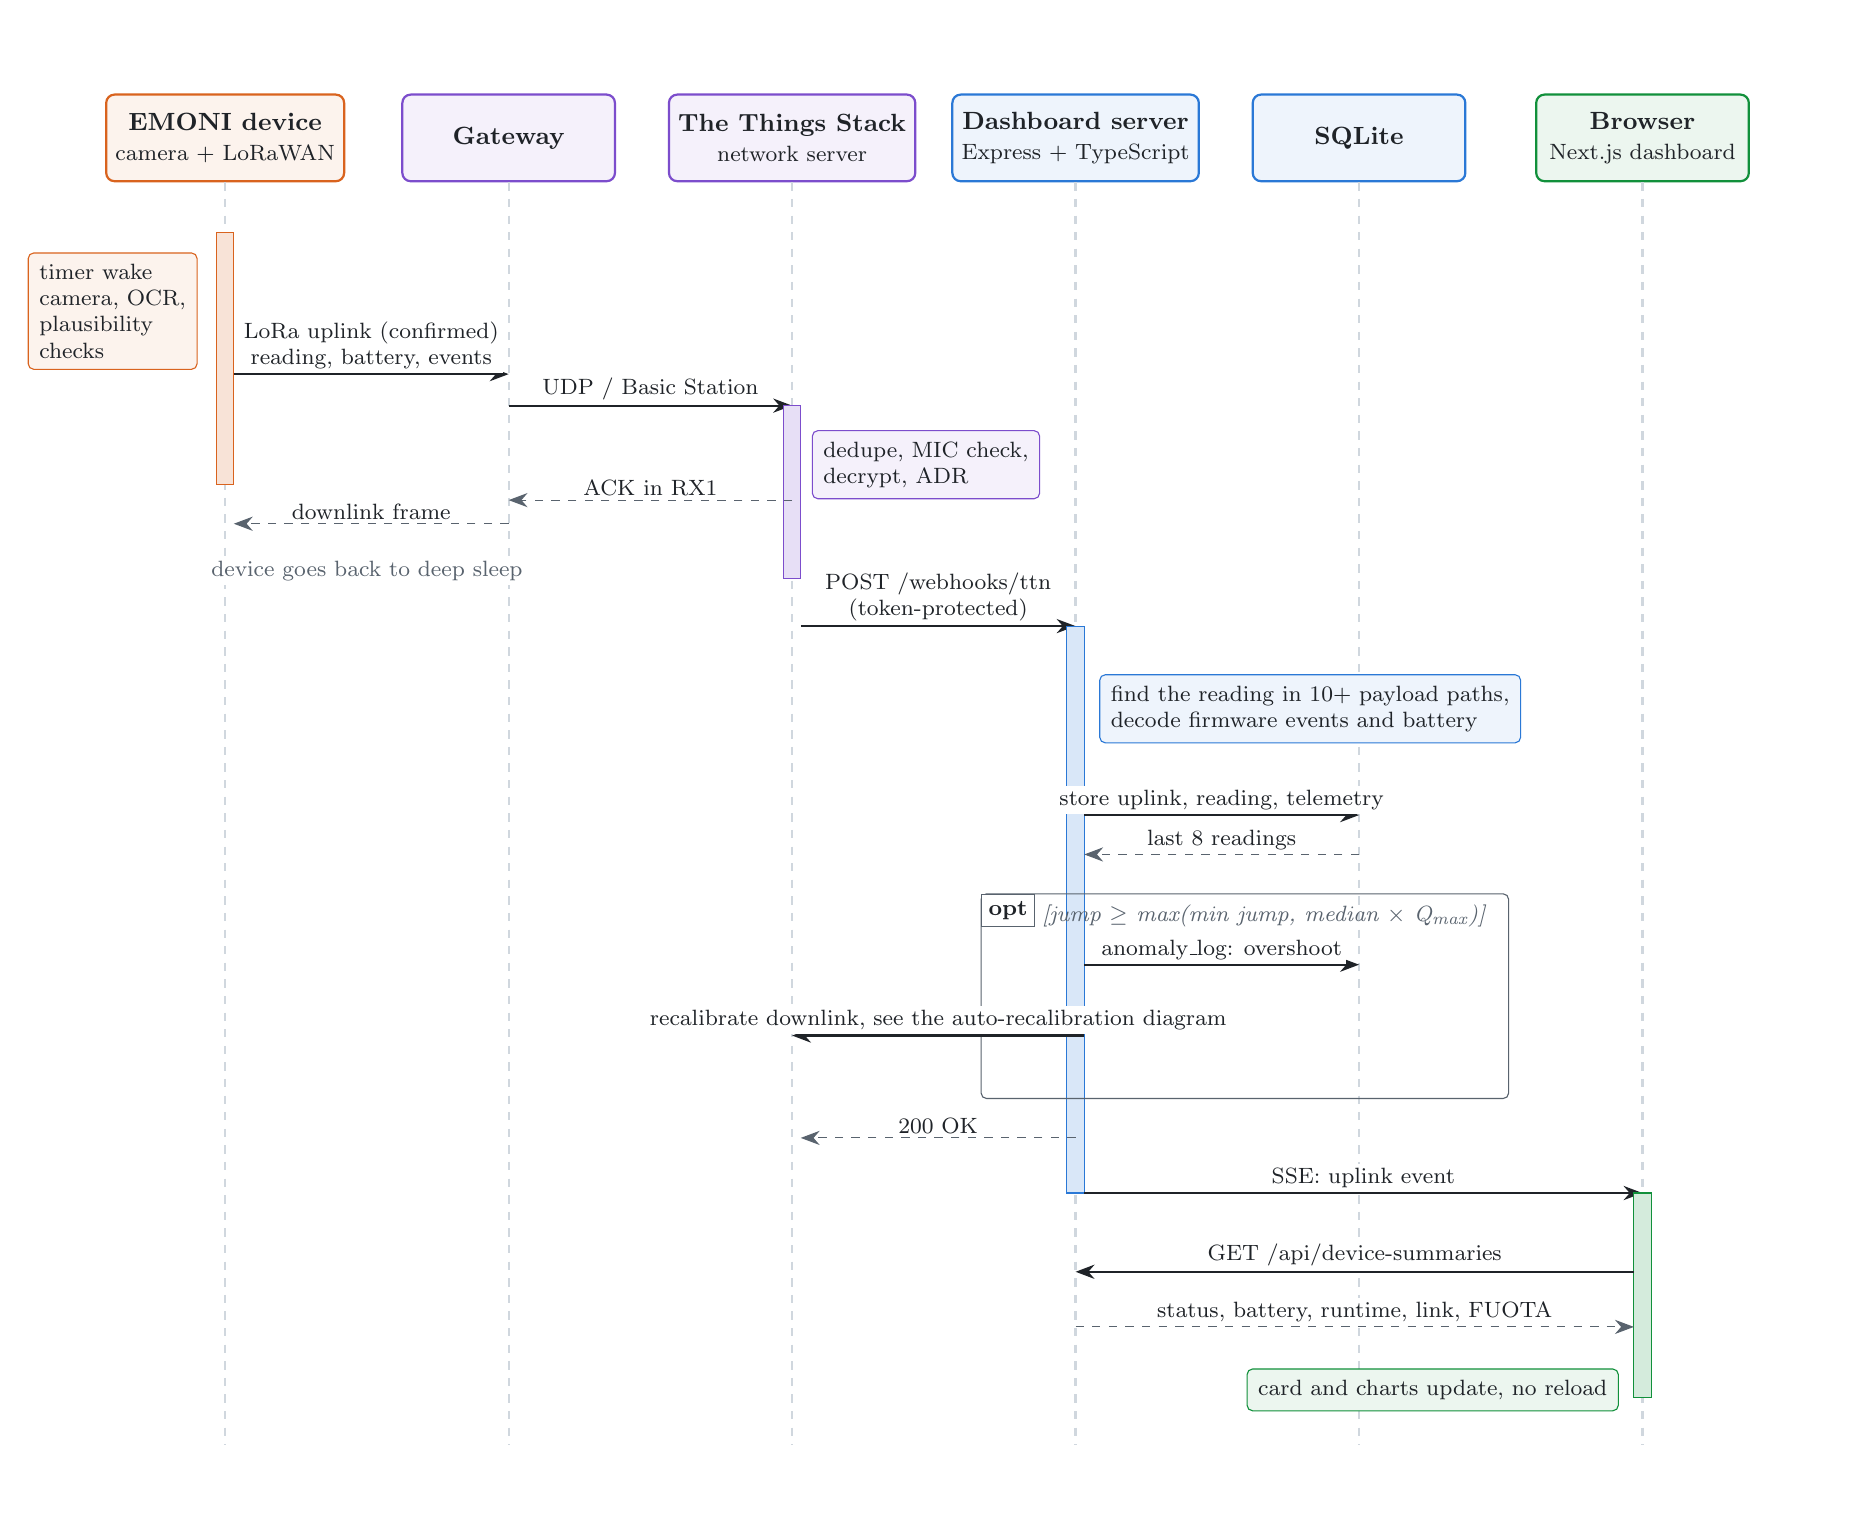
\begin{tikzpicture}[x=1cm,y=1cm]
\fill[white] (-2,1.4) rectangle (20.6,-17.2);
\def\B{-16.6}
\foreach \x/\n/\c/\t in {0/dev/eo/EMONI device\\{\footnotesize\mdseries camera + LoRaWAN},
                         3.6/gw/ep/Gateway,
                         7.2/ns/ep/The Things Stack\\{\footnotesize\mdseries network server},
                         10.8/srv/eb/Dashboard server\\{\footnotesize\mdseries Express + TypeScript},
                         14.4/db/eb/SQLite,
                         18.0/ui/eg/Browser\\{\footnotesize\mdseries Next.js dashboard}}{
  \node[head=\c] (\n) at (\x,0) {\t};
  \draw[life] (\n.south) -- (\x,\B);
}
% device wake
\draw[act=eo] (-0.11,-1.2) rectangle (0.11,-4.4);
\node[note=eo,anchor=east] at (-0.35,-2.2) {timer wake\\camera, OCR,\\plausibility\\checks};
\draw[msg] (0.11,-3.0) -- node[mlabel,above]{LoRa uplink (confirmed)\\reading, battery, events} (3.6,-3.0);
\draw[msg] (3.6,-3.4) -- node[mlabel,above]{UDP / Basic Station} (7.2,-3.4);
\draw[act=ep] (7.09,-3.4) rectangle (7.31,-5.6);
\node[note=ep,anchor=west] at (7.45,-4.15) {dedupe, MIC check,\\decrypt, ADR};
\draw[ret] (7.2,-4.6) -- node[mlabel,above]{ACK in RX1} (3.6,-4.6);
\draw[ret] (3.6,-4.9) -- node[mlabel,above]{downlink frame} (0.11,-4.9);
\node[mlabel,text=mute] at (1.8,-5.5) {device goes back to deep sleep};
% webhook
\draw[msg] (7.31,-6.2) -- node[mlabel,above]{POST /webhooks/ttn\\(token-protected)} (10.8,-6.2);
\draw[act=eb] (10.69,-6.2) rectangle (10.91,-13.4);
\node[note=eb,anchor=west] at (11.1,-7.25) {find the reading in 10+ payload paths,\\decode firmware events and battery};
\draw[msg] (10.91,-8.6) -- node[mlabel,above]{store uplink, reading, telemetry} (14.4,-8.6);
\draw[ret] (14.4,-9.1) -- node[mlabel,above]{last 8 readings} (10.91,-9.1);
% alt anomaly
\draw[frag] (9.6,-9.6) rectangle (16.3,-12.2);
\node[fraglabel] at (9.6,-9.6) {opt};
\node[font=\footnotesize\itshape,text=mute,anchor=north west] at (10.25,-9.62) {[jump $\geq$ max(min jump, median $\times$ Q\textsubscript{max})]};
\draw[msg] (10.91,-10.5) -- node[mlabel,above]{anomaly\_log: overshoot} (14.4,-10.5);
\draw[msg] (10.91,-11.4) -- node[mlabel,above]{recalibrate downlink, see the auto-recalibration diagram} (7.2,-11.4);
\draw[ret] (10.8,-12.7) -- node[mlabel,above]{200 OK} (7.31,-12.7);
% SSE
\draw[msg] (10.91,-13.4) -- node[mlabel,above]{SSE: uplink event} (18,-13.4);
\draw[act=eg] (17.89,-13.4) rectangle (18.11,-16.0);
\draw[msg] (17.89,-14.4) -- node[mlabel,above]{GET /api/device-summaries} (10.8,-14.4);
\draw[ret] (10.8,-15.1) -- node[mlabel,above]{status, battery, runtime, link, FUOTA} (17.89,-15.1);
\node[note=eg,anchor=east] at (17.7,-15.9) {card and charts update, no reload};
\end{tikzpicture}
\end{document}
